\chapter{Shot Boundary Detection}

Commonly, a video structure is as follows: The video is divided into scenes and each scene into one or more shots. A shot is a continuous frame sequence captured by a single camera action \cite{FormalStudyofSBD}. Some works introduce stories, that group semantically related scenes \cite{MethodsandChallengesinSBD}, or threads, that group similar shots, e.g. captured from the same camera point \cite{LearningContextualThreadModelSceneSegmentation}. Shots are, however, the most studied and the most used since shot detection is considered a fundamental step in video analysis. Information about shots is being exploited in video summarization \cite{Zhao_2018_CVPR}, video retrieval for advanced browsing and filtering \cite{LokocVBSJournal2018}, or even content-based copy detection \cite{Fuzzycolorhistogram}. However, information about the transitions is not available in the video format. Therefore, automated shot boundary detection methods need to be employed.

% A popular way to structure a video is by making use of a shot composition, where shots are delimited by transitions. Since information about the transitions is not available in the video format, automated shot boundary detection is an important step for video management and retrieval systems. For example, information about shots can be employed for video summarization, advanced browsing and filtering in known-item search tasks \cite{CobarzanSBHBLVB17,LokocBSMA18,Lokoc2019}.
% Shot changes can be either immediate (hard cuts) or gradual, the later spanning from basic linear interleaving of two shots over a certain number of video frames to more exotic geometric transformations from one shot to another one.
Any successful method must take into account that shot changes can be either immediate (hard cuts) or gradual. Common types of gradual transitions include dissolves (interleaving of two shots over a certain number of video frames), fade-ins and fade-outs (also considered as special types of dissolves where one shot is a blank image of a single color) and wipes (one shot slides from a side on top of the other shot). However, there are also many more exotic geometric transformations from one shot to another one.
%The later spanning from basic dissolves (interleaving of two shots over a certain number of video frames) to more exotic geometric transformations from one shot to another one. 
To make matters worse, shot boundary detectors must distinguish between shot transitions and sudden changes in a video caused by flashing light or partial occlusion of the scene by an object passing closer to the camera. Fast camera motion or motion of an object in the scene should also not be mistaken for a shot transition. This may indicate that some semantic representation of a scene is necessary to correctly segment a video.

Lastly, in some cases, a shot boundary is not a well-defined concept and question whether there is a transition may be subjective. Here we list some ambiguous cases and leave it for the reader to decide whether it should be a transition or not. Is a moment when captions are displayed at the end of a movie a transition? What if they raise from the bottom of the frame? A camera slowly enters a dark room -- is it fade-out? Newscast with two reporters side-by-side -- what if there is cut in a window of one reporter? Yet, with these examples, we only scratch the surface of the problem. Therefore, when used in the wild, shot boundary detection methods need to be tuned to eliminate these ambiguities based on a particular task at hand. % in case of computer generated content there are even more ambiguous scenarios.

% - news bar stays while shot changes, news bar changes while shot stays the same
% - what if the news two reporters side by side, at one cut is made, what if cut is performed in small picture-in-picture overlay?
% - camera enters dark room, is it fade out?
% - are captions shot transitions?




\section{Related work}

There has been a lot of research in shot boundary detection methods. The methods range from the most basic ones, that utilize only pixel-wise differences \cite{zhang93} effective for cut detection in stationary shots with a small number of moving objects, to more robust techniques that have been developed in the last years. Firstly, we list some of the `standard' methods not based on neural networks, further in the section deep learning approaches are discussed. For a more complete overview of the `standard' methods, we point the reader to some of many review studies available~\cite{MethodsandChallengesinSBD}.

\begin{figure}
    \centering
    \begin{tikzpicture}[
    font=\sffamily\scriptsize,
    table/.style={
        matrix of nodes,
        row sep=-\pgflinewidth,
        column sep=-\pgflinewidth,
        nodes={
            rectangle,
            draw=black,
            align=center,
            inner sep=0pt,
            minimum height=0.35cm,
            text width=0.35cm,
        },
        font=\sffamily\tiny,
        nodes in empty cells,
    }]
    \definecolor{Xcolor}{RGB}{0,0,0}
    
\node[inner sep=0pt] at (-4,0)
{\includegraphics[align=c,width=.2\textwidth]{img/transnetv2/IMG_20200307_191029_edited.jpg}};

    \matrix [table] at (0,0){
|[fill=Xcolor!  16]| & |[fill=Xcolor!   8]| & |[fill=Xcolor!   0]| & |[fill=Xcolor!   0]| & |[fill=Xcolor!   0]| & |[fill=Xcolor!   0]| & |[fill=Xcolor!   0]| & |[fill=Xcolor!   0]| \\
|[fill=Xcolor!  13]| & |[fill=Xcolor!  28]| & |[fill=Xcolor!   5]| & |[fill=Xcolor!   0]| & |[fill=Xcolor!   0]| & |[fill=Xcolor!   0]| & |[fill=Xcolor!   0]| & |[fill=Xcolor!   0]| \\
|[fill=Xcolor!   7]| & |[fill=Xcolor!  32]| & |[fill=Xcolor!  38]| & |[fill=Xcolor!   5]| & |[fill=Xcolor!   1]| & |[fill=Xcolor!   0]| & |[fill=Xcolor!   0]| & |[fill=Xcolor!   0]| \\
|[fill=Xcolor!   1]| & |[fill=Xcolor!  19]| & |[fill=Xcolor!  44]| & |[fill=Xcolor!  30]| & |[fill=Xcolor!   6]| & |[fill=Xcolor!   2]| & |[fill=Xcolor!   0]| & |[fill=Xcolor!   0]| \\
|[fill=Xcolor!   0]| & |[fill=Xcolor!   4]| & |[fill=Xcolor!  27]| & |[fill=Xcolor!  26]| & |[fill=Xcolor!   8]| & |[fill=Xcolor!   7]| & |[fill=Xcolor!   3]| & |[fill=Xcolor!   0]| \\
|[fill=Xcolor!   0]| & |[fill=Xcolor!   0]| & |[fill=Xcolor!   7]| & |[fill=Xcolor!  29]| & |[fill=Xcolor!  12]| & |[fill=Xcolor!   6]| & |[fill=Xcolor!  29]| & |[fill=Xcolor! 100]| \\
|[fill=Xcolor!   0]| & |[fill=Xcolor!   0]| & |[fill=Xcolor!   0]| & |[fill=Xcolor!  11]| & |[fill=Xcolor!  19]| & |[fill=Xcolor!   2]| & |[fill=Xcolor!   5]| & |[fill=Xcolor!  35]| \\
|[fill=Xcolor!   0]| & |[fill=Xcolor!   0]| & |[fill=Xcolor!   0]| & |[fill=Xcolor!   0]| & |[fill=Xcolor!   1]| & |[fill=Xcolor!   0]| & |[fill=Xcolor!   0]| & |[fill=Xcolor!   0]| \\
    };
    
    \node[] at (0, 1.7) {\footnotesize RGB Histogram};
    \node[rotate=90] at (-1.7, 0) {Red};
    \node[] at (0, -1.7) {Blue};
    
        \matrix [table] at (4,0){
|[fill=Xcolor!   0]| & |[fill=Xcolor!   0]| & |[fill=Xcolor!   7]| & |[fill=Xcolor!  17]| & |[fill=Xcolor!  10]| & |[fill=Xcolor!   6]| & |[fill=Xcolor!   2]| & |[fill=Xcolor!   1]| \\
|[fill=Xcolor!   0]| & |[fill=Xcolor!   0]| & |[fill=Xcolor!   0]| & |[fill=Xcolor!   0]| & |[fill=Xcolor!   0]| & |[fill=Xcolor!   0]| & |[fill=Xcolor!   0]| & |[fill=Xcolor!   0]| \\
|[fill=Xcolor!   0]| & |[fill=Xcolor!   0]| & |[fill=Xcolor!   0]| & |[fill=Xcolor!   0]| & |[fill=Xcolor!   0]| & |[fill=Xcolor!   0]| & |[fill=Xcolor!   0]| & |[fill=Xcolor!   0]| \\
|[fill=Xcolor!   0]| & |[fill=Xcolor!  36]| & |[fill=Xcolor! 100]| & |[fill=Xcolor!   4]| & |[fill=Xcolor!   7]| & |[fill=Xcolor!   4]| & |[fill=Xcolor!   1]| & |[fill=Xcolor!   1]| \\
|[fill=Xcolor!   0]| & |[fill=Xcolor!  54]| & |[fill=Xcolor!  63]| & |[fill=Xcolor!  34]| & |[fill=Xcolor!  17]| & |[fill=Xcolor!   9]| & |[fill=Xcolor!   6]| & |[fill=Xcolor!   5]| \\
|[fill=Xcolor!   0]| & |[fill=Xcolor!   2]| & |[fill=Xcolor!  42]| & |[fill=Xcolor!  78]| & |[fill=Xcolor!  40]| & |[fill=Xcolor!  16]| & |[fill=Xcolor!   7]| & |[fill=Xcolor!   6]| \\
|[fill=Xcolor!   0]| & |[fill=Xcolor!   0]| & |[fill=Xcolor!   0]| & |[fill=Xcolor!   0]| & |[fill=Xcolor!   0]| & |[fill=Xcolor!   0]| & |[fill=Xcolor!   0]| & |[fill=Xcolor!   0]| \\
|[fill=Xcolor!   0]| & |[fill=Xcolor!   0]| & |[fill=Xcolor!   0]| & |[fill=Xcolor!   0]| & |[fill=Xcolor!   0]| & |[fill=Xcolor!   0]| & |[fill=Xcolor!   0]| & |[fill=Xcolor!   0]| \\    };

    \node[] at (4, 1.7) {\footnotesize HSV Histogram};
    \node[rotate=90] at (2.3, 0) {Hue};
    \node[] at (4, -1.7) {Saturation};

    \end{tikzpicture}
    \caption[Visualization of RGB and HSV histogram of a single image]{Visualization of RGB and HSV histogram of a single image. The intensity of each bin indicates a number of image pixels with the given color. Third dimension depicting green or value respectively is not shown.}
    \label{fig:colorhist}
\end{figure}

\begin{description}[labelwidth=1em, leftmargin=!]
    \item \textbf{Color histograms.} Widely used technique for shot boundary detection. It is based on computing histograms for each frame and thresholding distance between consecutive histogram representations. Instead of traditional RGB histograms, some works use HSV histograms to reduce disturbance in illumination \cite{LingGeneralMethodforSBD} (comparison shown in Figure \ref{fig:colorhist}) or LAB histograms since they better approximate the way humans perceive color \cite{Fuzzycolorhistogram}. To improve the detection rate, frames can be divided into multiple patches with histograms computed for each patch \cite{Cineast}. Also, instead of a distance-based comparison, $\chi^2$ comparison of color histograms is sometimes used.

    \item \textbf{Feature based methods.} One of the earliest feature-based methods computes changes in edges of subsequent frames \cite{zabih1995feature}. It is based on observation, that during transition, new edges appear far from the locations of old edges and vice versa. However, the work of Rainer Lienhart \cite{LienhartComparison1998} shows that the method brings no significant improvements over color histograms. Nonetheless, edge-like features are utilized in shot boundary detector by Shao et al. \cite{shao15} where histogram of gradients is used as a secondary method to HSV histogram. Apostolidis et al. \cite{apostolidis14} take advantage of scale and rotation invariant SURF descriptors \cite{surf} to measure differences between a pair of frames.
    
    \item \textbf{Clustering.} Given a feature vector for each frame such as a color histogram or more recently a vector computed by a neural network, a clustering algorithm can be run to determine shot boundaries. Verma et al. \cite{VermaClustering} use a special form of hierarchical clustering to join consecutive frames into shots while Baraldi et al. \cite{BaraldiScenes} utilizes clustering to determine which shots belong to a particular scene.

    \item \textbf{Support vector machines} (SVMs)\textbf{.} Given a set of adjacent frame similarities, it may seem arbitrary to select a threshold value that decides whether there is a transition or not, especially for gradual transitions. In the work of Chasanis et al. \cite{ChasanisSVM}, SVMs are trained on a sliding window of neighboring frame similarities to predict shot boundaries instead of using a simple threshold. Tsamoura et al. \cite{TsamouraSVM} increase the chance of detection by adding new similarity/distance metrics based, for example, on Color Coherence Vectors \cite{pass1997comparing} to the SVM's input feature vector.

    \item \textbf{Flash detection.} Commonly, some videos contain either photographic\linebreak[4] flashes or overexposed frames due to change in illumination of a camera sensor, e.g. when a light is turned on. It is not uncommon to perform a post-processing step that compares frames or their features such as luminance values that are adjacent to potential shot boundary \cite{kawai2007shot}. If there is no significant change observed in the adjacent frames, probably a flash occurred.

    \item \textbf{Other false positive suppression methods.} Motion in a scene or motion of a camera can result in many false positives. Camera motion estimation \cite{muhling2007university} or optical flow \cite{ayache2006clips} methods are used to reduce the number of false alarms, especially for gradual transitions. When not using SVMs, a threshold for transition detection has to be set. Work of Yeo et al. \cite{Yeo1995Rapid} sets the threshold adaptively since using the same threshold for different video genres can result in many false positives in one and false negatives in another.
\end{description}

Between years 2001 and 2007 there had been automatic shot boundary detection (SBD) challenge held annually at TRECVid (TREC Video Retrieval Evaluation) \cite{SevenyearsofTRECVid} with teams utilizing many of the described techniques; however, it was discontinued due to no observed improvements over the last years of the challenge. Significant improvements came with deep learning revolution when, for example, the work of Hassanien et al. \cite{Hassanien17} achieved on the RAI dataset F1 score of 0.94 improving previous state-of-the-art by 0.1 from 0.84 \cite{Baraldi15,apostolidis14}. Therefore, the next paragraphs introduce deep learning approaches towards the shot boundary detection.

\subsection{Deep Learning Methods}

\begin{figure}[h]
    \centering
    \input{img/convvis/earlyfusion}\hspace{10pt}
    \input{img/convvis/latefusion}
    \begin{tikzpicture}[scale=.33,every node/.style={minimum size=1cm},on grid]
\definecolor{base01}{RGB}{88,110,117}
\definecolor{base02}{RGB}{7,54,66}
\definecolor{base03}{RGB}{0,43,54}
\definecolor{cyan}{RGB}{195, 236, 255}
\definecolor{blue}{RGB}{208, 240, 192}

    \begin{scope}[xshift=-4.5cm, yshift=-2.25cm, node/.append style={yslant=0.5,xslant=-0.7},
                    yslant=0.5,xslant=-0.7]
        \draw[step=10mm, base03, dashed, thick] (0,0) grid (4,4);
        \draw[draw=base03, fill=blue, thick] (0,0) rectangle (1,1);
        \draw[draw=base03, fill=blue, thick] (0,1) rectangle (1,2);
        \draw[draw=base03, fill=blue, thick] (0,2) rectangle (1,3);
        \draw[draw=base03, fill=blue, thick] (0,3) rectangle (1,4);
        \draw[draw=base03, fill=blue, thick] (1,0) rectangle (2,1);
        \draw[draw=base03, fill=blue, thick] (1,1) rectangle (2,2);
        \draw[draw=base03, fill=blue, thick] (1,2) rectangle (2,3);
        \draw[draw=base03, fill=blue, thick] (1,3) rectangle (2,4);
        \draw[draw=base03, fill=blue, thick] (2,0) rectangle (3,1);
        \draw[draw=base03, fill=blue, thick] (2,1) rectangle (3,2);
        \draw[draw=base03, fill=blue, thick] (2,2) rectangle (3,3);
        \draw[draw=base03, fill=blue, thick] (2,3) rectangle (3,4);
        \draw[draw=base03, fill=blue, thick] (3,0) rectangle (4,1);
        \draw[draw=base03, fill=blue, thick] (3,1) rectangle (4,2);
        \draw[draw=base03, fill=blue, thick] (3,2) rectangle (4,3);
        \draw[draw=base03, fill=blue, thick] (3,3) rectangle (4,4);


        \foreach \x in { 0,\number\numexpr 0+1,...,\number\numexpr 3-1 } {
            \foreach \y in { 1,\number\numexpr 1+1,...,\number\numexpr 4-1 } {
                \draw[fill=base02, opacity=0.4] (\x,\y) rectangle
                                        (\x+1,\y+1);
            }
        }
        \draw[step=10mm, base03, thick] (0, 1) grid
                                        (3, 4);
                                        
        \coordinate (BL3) at (0,1);
        \coordinate (BR3) at (3,1);
        \coordinate (TL3) at (0,4);
        \coordinate (TR3) at (3,4);
    \end{scope}
    
        \begin{scope}[xshift=4.5cm, yshift=2.25cm, node/.append style={yslant=0.5,xslant=-0.7},
                    yslant=0.5,xslant=-0.7]
        \draw[step=10mm, base03, dashed, thick] (0,0) grid (4,4);
        \draw[draw=base03, fill=blue, thick] (0,0) rectangle (1,1);
        \draw[draw=base03, fill=blue, thick] (0,1) rectangle (1,2);
        \draw[draw=base03, fill=blue, thick] (0,2) rectangle (1,3);
        \draw[draw=base03, fill=blue, thick] (0,3) rectangle (1,4);
        \draw[draw=base03, fill=blue, thick] (1,0) rectangle (2,1);
        \draw[draw=base03, fill=blue, thick] (1,1) rectangle (2,2);
        \draw[draw=base03, fill=blue, thick] (1,2) rectangle (2,3);
        \draw[draw=base03, fill=blue, thick] (1,3) rectangle (2,4);
        \draw[draw=base03, fill=blue, thick] (2,0) rectangle (3,1);
        \draw[draw=base03, fill=blue, thick] (2,1) rectangle (3,2);
        \draw[draw=base03, fill=blue, thick] (2,2) rectangle (3,3);
        \draw[draw=base03, fill=blue, thick] (2,3) rectangle (3,4);
        \draw[draw=base03, fill=blue, thick] (3,0) rectangle (4,1);
        \draw[draw=base03, fill=blue, thick] (3,1) rectangle (4,2);
        \draw[draw=base03, fill=blue, thick] (3,2) rectangle (4,3);
        \draw[draw=base03, fill=blue, thick] (3,3) rectangle (4,4);


        \foreach \x in { 0,\number\numexpr 0+1,...,\number\numexpr 3-1 } {
            \foreach \y in { 1,\number\numexpr 1+1,...,\number\numexpr 4-1 } {
                \draw[fill=base02, opacity=0.4] (\x,\y) rectangle
                                        (\x+1,\y+1);
            }
        }
        \draw[step=10mm, base03, thick] (0, 1) grid
                                        (3, 4);
                                        
        \coordinate (BL2) at (0,1);
        \coordinate (BR2) at (3,1);
        \coordinate (TL2) at (0,4);
        \coordinate (TR2) at (3,4);
    \end{scope}
    
    \begin{scope}[node/.append style={yslant=0.5,xslant=-0.7},
                    yslant=0.5,xslant=-0.7]
        \draw[step=10mm, base03, dashed, thick] (0,0) grid (4,4);
        \draw[draw=base03, fill=blue, thick] (0,0) rectangle (1,1);
        \draw[draw=base03, fill=blue, thick] (0,1) rectangle (1,2);
        \draw[draw=base03, fill=blue, thick] (0,2) rectangle (1,3);
        \draw[draw=base03, fill=blue, thick] (0,3) rectangle (1,4);
        \draw[draw=base03, fill=blue, thick] (1,0) rectangle (2,1);
        \draw[draw=base03, fill=blue, thick] (1,1) rectangle (2,2);
        \draw[draw=base03, fill=blue, thick] (1,2) rectangle (2,3);
        \draw[draw=base03, fill=blue, thick] (1,3) rectangle (2,4);
        \draw[draw=base03, fill=blue, thick] (2,0) rectangle (3,1);
        \draw[draw=base03, fill=blue, thick] (2,1) rectangle (3,2);
        \draw[draw=base03, fill=blue, thick] (2,2) rectangle (3,3);
        \draw[draw=base03, fill=blue, thick] (2,3) rectangle (3,4);
        \draw[draw=base03, fill=blue, thick] (3,0) rectangle (4,1);
        \draw[draw=base03, fill=blue, thick] (3,1) rectangle (4,2);
        \draw[draw=base03, fill=blue, thick] (3,2) rectangle (4,3);
        \draw[draw=base03, fill=blue, thick] (3,3) rectangle (4,4);


        \foreach \x in { 0,\number\numexpr 0+1,...,\number\numexpr 3-1 } {
            \foreach \y in { 1,\number\numexpr 1+1,...,\number\numexpr 4-1 } {
                \draw[fill=base02, opacity=0.4] (\x,\y) rectangle
                                        (\x+1,\y+1);
            }
        }
        \draw[step=10mm, base03, thick] (0, 1) grid
                                        (3, 4);
        \coordinate (BL) at (0,1);
        \coordinate (BR) at (3,1);
        \coordinate (TL) at (0,4);
        \coordinate (TR) at (3,4);
    \end{scope}
    
    \begin{scope}[xshift=0cm, yshift=5cm,
                    every node/.append style={yslant=0.5,xslant=-0.7},
                    yslant=0.5,xslant=-0.7]
        \draw (BL) -- (0,1) (BR) -- (1,1)
              (TL) -- (0,2) (TR) -- (1,2);
        \draw (BL2) -- (0,1) (BR2) -- (1,1)
              (TL2) -- (0,2) (TR2) -- (1,2);
        \draw (BL3) -- (0,1) (BR3) -- (1,1)
              (TL3) -- (0,2) (TR3) -- (1,2);
        \draw[fill=cyan] (0,0) rectangle (2,2);
        \draw[step=10mm, base03, thick] (0,0) grid (2,2);
        \draw[fill=base02, opacity=0.4] (0,1) rectangle
                                        (1,2);
        \draw[base03, thick] (0,1) rectangle (1,2);
    \end{scope}

    \begin{scope}[xshift=4.5cm, yshift=7.25cm,
                    every node/.append style={yslant=0.5,xslant=-0.7},
                    yslant=0.5,xslant=-0.7]
        \draw[fill=cyan] (0,0) rectangle (2,2);
        \draw[step=10mm, base03, thick] (0,0) grid (2,2);
    \end{scope}
    \begin{scope}[xshift=-4.5cm, yshift=2.75cm,
                    every node/.append style={yslant=0.5,xslant=-0.7},
                    yslant=0.5,xslant=-0.7]
        \draw[fill=cyan] (0,0) rectangle (2,2);
        \draw[step=10mm, base03, thick] (0,0) grid (2,2);
    \end{scope}
\end{tikzpicture}
    \caption[Comparison of early fusion, late fusion and 3D convolutions]{Comparison of early fusion (left), late fusion (middle) and 3D convolutions (right). In the case of late fusion, some aggregation over frames must be done to capture temporal information (not shown).}
    \label{fig:3dFusionApproches}
\end{figure}

Exciting results of Krizhevsky et al. \cite{AlexNet} sparked a great interest in image classification research using convolutional neural networks. These networks, trained in a fully supervised manner, learn a rich semantic representation that can be repurposed to novel generic tasks \cite{donahue2014decaf}.
Therefore, one of the first deep learning SBD works \cite{Xu2016AlexNetForSBD} revolves around utilizing this readily available `deep' representation. It uses FC-6 features from AlexNet neural network \cite{AlexNet} and employs cosine similarity between frames' features in the decision process, whether there is transition.

To utilize temporal information in a neural network directly, many approaches have been developed. The \textit{late fusion} \cite{Karpathy_2014_CVPR} approach extracts features from individual images. The features are then merged, for example, by averaging them over time or concatenating a fixed number of them. Fully connected layers are placed atop the aggregated representation. The \textit{early fusion} approach stacks $N$ (subsequent) frames in channel dimension therefore increasing number of channels in input from three (RGB) to $3\times N$. \textit{Two-stream} architecture \cite{SimonyanTwoStream} utilizes two networks -- one for single frame and another one that processes optical flow information from multiple adjacent frames. Figure \ref{fig:3dFusionApproches} shows a visual comparison between these approaches.

However, all of the above approaches utilize only 2D convolutions. First widely popular network utilizing 3D convolutions C3D (Figure \ref{fig:c3d_network}) introduced in the work of Tran et al. \cite{Tran_2015_C3D} showed modest improvements over 2D approaches. Bigger I3D network \cite{Carreira_2017_CVPR}, closely resembling 2D convolutional network InceptionV1 \cite{Szegedy_2015_CVPR}, brought further improvements and also showed the benefits of the Two-Stream approach still hold even for 3D convolutional networks. Other improvements were achieved by separation of 3D convolutions into spatial-only and temporal-only convolutions \cite{Xie_2018_ECCV, Tran_2018_CVPR}.

\begin{figure}[t]
    \centering
    \begin{tikzpicture}[
    font=\sffamily\scriptsize,
    box/.style={
    	draw,
    	minimum width=0.7cm,
    	minimum height=0.4cm,
    	rounded corners=2, inner sep=2pt, align=center, anchor=north,
    	text width=1.7cm
    }, pil/.style={
    	-{Stealth[scale=.5]},
    	rounded corners=5pt,
    	line width=1pt
    }]
    \definecolor{my-green}{RGB}{208, 240, 192}
    \definecolor{my-yellow}{RGB}{247, 231, 206}
    \definecolor{my-blue}{RGB}{195, 236, 255}

    \begin{scope}[rotate=90,box/.append style={rotate=90}]

    \node[box, fill=my-green] (layer1) at (0,0)    {Conv 3$\times$3$\times$3\\[-2pt]{\tiny 64 filters}};
    \node[box, fill=my-yellow] (pool1) at (0,-0.8) {Max pooling\\1$\times$2$\times$2};
    \node[box, fill=my-green] (layer2) at (0,-1.7) {Conv 3$\times$3$\times$3\\[-2pt]{\tiny 128 filters}};
    \node[box, fill=my-yellow] (pool2) at (0,-2.5) {Max pooling\\2$\times$2$\times$2};
    \node[box, fill=my-green] (layer3) at (0,-3.4) {Conv 3$\times$3$\times$3\\[-2pt]{\tiny 256 filters}};
    \node[box, fill=my-green] (layer4) at (0,-4.2) {Conv 3$\times$3$\times$3\\[-2pt]{\tiny 256 filters}};
    \node[box, fill=my-yellow] (pool3) at (0,-5.0) {Max pooling\\2$\times$2$\times$2};
    \node[box, fill=my-green] (layer5) at (0,-5.9) {Conv 3$\times$3$\times$3\\[-2pt]{\tiny 512 filters}};
    \node[box, fill=my-green] (layer6) at (0,-6.7) {Conv 3$\times$3$\times$3\\[-2pt]{\tiny 512 filters}};
    \node[box, fill=my-yellow] (pool4) at (0,-7.5) {Max pooling\\2$\times$2$\times$2};
    \node[box, fill=my-green] (layer7) at (0,-8.4) {Conv 3$\times$3$\times$3\\[-2pt]{\tiny 512 filters}};
    \node[box, fill=my-green] (layer8) at (0,-9.2) {Conv 3$\times$3$\times$3\\[-2pt]{\tiny 512 filters}};
    \node[box, fill=my-yellow] (pool5) at (0,-10) {Max pooling\\2$\times$2$\times$2};
    \node[box, anchor=north, fill=my-blue] (dense1) at (0,-10.9) {Dense 4096};
    \node[box, anchor=north, fill=my-blue] (dense2) at (0,-11.5) {Dense 4096};
    \node[box, anchor=north, text width=1.2cm] (softmax) at (0,-12.1) {Softmax};
    
    \draw[pil] (layer1) -- (pool1);
    \draw[pil] (pool1) -- (layer2);
    
    \draw[pil] (layer2) -- (pool2);
    \draw[pil] (pool2) -- (layer3);
    
    \draw[pil] (layer3) -- (layer4);
    \draw[pil] (layer4) -- (pool3);
    \draw[pil] (pool3) -- (layer5);
    
    \draw[pil] (layer5) -- (layer6);
    \draw[pil] (layer6) -- (pool4);
    \draw[pil] (pool4) -- (layer7);
    
    \draw[pil] (layer7) -- (layer8);
    \draw[pil] (layer8) -- (pool5);
    \draw[pil] (pool5) -- (dense1);
    
    \draw[pil] (dense1) -- (dense2);
    \draw[pil] (dense2) -- (softmax);
    \end{scope}
    \end{tikzpicture}
    \caption[C3D architecture]{C3D architecture by Tran et al. \cite{Tran_2015_C3D}. C3D net has 8~convolution, 5~max-pooling, and 2~fully connected layers, followed by a softmax output layer.}
    \label{fig:c3d_network}
\end{figure}

% introduced in the work of Tran et al. \cite{Learning Spatiotemporal Features with 3D Convolutional Networks} learns features with 3D convolutions showing modest improvements over 2D approaches. Further improvements were achieved by bigger I3D network. While C3D network can be thought of as 3D version of AlexNet, I3D network resembles Inception V1 architecture. Authors of I3D show that even when using 3D convolutions the Two-Stream aproach is still beneficial.


Using 3D convolutions for shot boundary detection has been popularized by Gygli \cite{Gygli18} and Hassanien et al. \cite{Hassanien17}. The later work introduces DeepSBD framework consisting of a CNN-based classification step, a merging step, and a post-processing step. The network, based on C3D architecture, takes 16 subsequent frames and predicts whether the segment contains sharp or gradual transition. The logits are, however, not used directly, but they are fed to an SVM classifier to give a labeling estimate. Further, consecutive segments with the same labeling are merged, and Bhattacharyya distance between color histograms of the first and the last frame of the proposed transition segment is computed. If the distance is small, the segment is considered as false positive and removed from a set of transitions.

The work of Gygli removes all post-processing steps by using only predictions from a 3D convolutional network. The network consists of 5 convolutional layers with a much smaller number of parameters than C3D. It takes 10 subsequent frames and predicts whether there is a transition between the middle frames. Because of the fully convolutional nature, the network can be stretched to take $N$ frames and produce output for the middle $N-9$ frames eliminating the need for processing most of the frames multiple times.  Further, this approach can localize the exact position of a transition, which is impossible in DeepSBD. However, reported performance is worse than the one reported by Hassanien et al.

\subsection{Datasets}
The above mentioned deep learning methods all rely on large annotated datasets. Since most of the available datasets are small and also used for evaluation, both Gygli \cite{Gygli18} and Hassanien et al. \cite{Hassanien17} overcome the need for the large dataset by generating synthetic training examples. Both works generate sharp transitions (hard cuts), dissolves, and simple horizontal wipes. The DeepSBD system further enriches a set of possible transitions by non-linearly interleaving dissolves and more complex wipes. Gygli adds artificial flashes to the non-transition sequences to make the network invariant to these kinds of changes.

For evaluation TRECVid SBD datasets are commonly used; however, they are old and publicly unavailable. A small, manually annotated dataset of broadcasting videos, mainly documentaries and talk shows from the archive of Italian TV station Rai Scuola \cite{Baraldi15}, has been used by many works. Further, the same authors released manually annotated shot and scene boundaries for all 11 episodes of the BBC educational TV series Planet Earth \cite{BaraldiScenes}. The whole dataset contains around 4900 shots and 670 scenes. Recently, new database ClipShots \cite{Tang2018} was released containing 4039 online videos with manually double annotated 128636 cut transitions and 38120 gradual transitions. The dataset contains videos from Youtube and Weibo covering more than 20 categories, including sports, TV shows, animals, etc. with hand-held camera vibrations, large object motions, and occlusion. Its test set consists of 500 videos with 5876 cut transitions and 2422 gradual transitions.

The authors of the ClipShots dataset also introduce their system based on a three-step pipeline. Firstly, SqueezeNet \cite{SqueezeNet} features for each frame are used to compute similarities between frames to reduce the number of candidates for transitions. A cut detector is applied to the transition candidates, and, in the end, if no cut transition is detected, a gradual detector is applied. For the cut detector, either C3D network or 2D ResNet-50 with the input of 6 concatenated subsequent frames is used, with the latter achieving better results. For gradual transition detection, both the DeepSBD-like system and a 3D version of ResNet-18 \cite{Hara_2018_CVPR} are tested. The version with ResNet performs per-frame classification as well as transition regression similar to region proposal in object detection. According to the authors, their ResNet based system outperforms DeepSBD\footnote{However, the only code provided by the authors is the reimplementation of DeepSBD, which contains an evaluation script that does not account for double detection of transitions and possibly other errors. Therefore, the reported results should be taken with a grain of salt.}.

%The goal of the shot boundary detection is to temporally segment a video into shots. To determine the shot boundary, one of the first methods utilized thresholded pixel differences \cite{zhang93} effective for stationary shots with a small number of moving objects. Since then, more robust techniques to compare images were developed based on local color histograms, color coherence vectors \cite{Pass1997} or SIFT features. The work of Shao et al. \cite{shao15} utilizes HSV and gradient histograms for shot boundary detection, Apostolidis et al. \cite{apostolidis14} use not only the histogram but also a set of SURF descriptors to detect the differences between a pair of frames. Other approaches revolve around edge information \cite{Huan2008} or motion vectors \cite{amel10}. 
%With the advent of deep learning, new methods for shot detection using convolutional neural networks (CNN) emerged. Baraldi et al. \cite{Baraldi15} utilize spectral clustering given a set of features for every frame extracted by a deep siamese network. Recently, Gygli \cite{Gygli18} used a relatively shallow neural network with 3D convolutions with the third dimension over time. Even though 3D convolutions significantly increase computational complexity and memory requirements over standard 2D convolutions due to the added dimension, Gygli has beaten the previous approach in accuracy and speed as well. Another approach by Hassanien et al. \cite{Hassanien17} also uses 3D CNN however its output is fed through SVM classifier and further postprocessing is done to reduce false alarms of gradual transitions through a histogram-driven temporal differencing.
%Our work partially overcomes problem of computationally hungry 3D convolutions when a large field of view is required to cope with long gradual transitions by using dilated convolutions over the time dimension, which had been proven useful in speech generation task \cite{oord16}.
%The deep learning approaches revolve around the need for large annotated datasets. Until recently \cite{Tang2018}, the size of publicly available datasets for SBD was the limiting factor. Fortunately, synthetic training data can be easily generated from virtually any video content by interleaving randomly selected sequences from different videos as is done in \cite{Gygli18} and others. The downside of this method is, however, that the real data can contain cuts between shots of the same scene which rarely occur in the synthetic data sets due to the nature how they are generated.







\clearpage
\section{TransNet}\label{sec:transnetv1}
This section introduces TransNet, scalable architecture for shot boundary detection introduced in \cite{soucek2019transnet,LokocMM2019}. The network features multiple dilated 3D convolutional operations per layer and achieves state-of-the-art results on the RAI data\-set~\cite{Baraldi15}. Firstly, we describe the model architecture, then we introduce performed experiments and report their results. Further, in the next section, improvements to the TransNet are presented. Some texts in this section overlap with our paper~\cite{soucek2019transnet}. These texts were written by the author of this thesis.


\subsection{Model Architecture}

The proposed TransNet architecture (Figure \ref{fig:nn_architecture}) is inspired by many very successful convolutional architectures for image classification \cite{AlexNet} or action recognition~\cite{Tran_2015_C3D}. Commonly these architectures feature a layer or a cell that consists of a single or multiple convolutional operations, each with different parameters. These cells are stacked to form the whole network. To reduce the spatial and temporal resolution of the network, reduction cells are included in between some of the standard cells. These consist of either pooling operations or convolutions with greater strides. TransNet is built upon these concepts with the only exception of temporal pooling, which is not applied to precisely localize shot boundaries on the level of individual frames. In general, the network takes a sequence of $N$ consecutive video frames and applies series of 3D convolutions returning a prediction for every frame in the input. Each prediction expresses how likely a given frame is a shot boundary.

Convolutional neural networks for video-related tasks such as C3D \cite{Tran_2015_C3D} introduced for action recognition employ many 3D convolution layers. However, a big problem with 3D convolutions is that even minimal $3\times 3\times 3$ convolutions can be prohibitively expensive. Yet it is not uncommon for a transition to span across dozens of frames; therefore, it is necessary to ensure a wide temporal field of view for the convolution operations, which is computationally even more expensive. Also, the larger the convolutional kernels are, the bigger the number of parameters is, which can result in over-fitting, especially since shot boundary datasets are rather small compared to, for example, large image classification datasets such as ImageNet.

TransNet solves this problem by utilizing dilated convolutions that have been successfully applied to many tasks ranging from image segmentation \cite{yu2015multi} to audio generation \cite{WaveNet}. The main building layer of the model, dubbed Dilated Deep CNN (DDCNN) cell, is designed to have a large field of view with a minimal number of parameters while still maintaining the ability to capture a change in two consecutive frames. The cell consists of four 3D $3\times3\times3$ convolutional operations each with $N_{in}\times 3\times 3\times 3\times N_{out} / 4$ learnable parameters where $N_{in}$ is number of filters from the previous layer and $N_{out}$ is number of filters outputted by the cell. Each of the four convolutions employs different dilation rates for the temporal dimension. The rates are 1, 2, 4, and 8, i.e. the first convolution is standard $3\times3\times3$ convolution that looks one frame to the left and one frame to the right, the last convolution looks at the eighth frame to the left and the eighth frame to the right.
The four convolutional outputs are concatenated, creating a representation with $N_{out}$ filters. Compared to standard convolution with the same number of output filters and the same field of view, the DDCNN cell achieves more than a six-fold reduction in the number of learnable parameters.

Multiple DDCNN cells on top of each other, followed by spatial max pooling, form a Stacked DDCNN block. The TransNet consists of multiple SDDCNN blocks, every next block operating on smaller spatial resolution but with a larger number of filters, further increasing the expressive power and the receptive field of the network.
Two fully connected layers refine the features extracted by the convolutional layers and predict a possible shot boundary for every frame representation independently (layer weights are shared). ReLU activation function is used in all layers, with the only exception of the last fully connected layer with softmax output. Stride 1 and the `same' padding is employed in all convolutional layers.


\begin{figure}[t]
    \centering
    \begin{tikzpicture}[
    font=\sffamily\scriptsize,
    box/.style={
    	draw,
    	minimum width=0.7cm,
    	minimum height=0.4cm,
    	rounded corners=2, inner sep=2pt, align=center, anchor=north,
    	text width=1.7cm
    }, pil/.style={
    	-{Stealth[scale=.5]},
    	rounded corners=5pt,
    	line width=1pt
    }]
    \definecolor{my-green}{RGB}{208, 240, 192}
    \definecolor{my-yellow}{RGB}{247, 231, 206}
    \definecolor{my-blue}{RGB}{195, 236, 255}
    \definecolor{my-gray}{RGB}{251, 251, 251}
    \definecolor{my-gray2}{RGB}{245, 245, 245}
    
    
    \node[box, draw=none, text width=3cm] (input) at (0,3.5) {Input\\$N \times width \times height \times 3$};
    
    \node[box, draw=lightgray, text width=8.2cm, text height=2.9cm, fill=my-gray] at (0,2.6) {};

    \node[box, draw=lightgray, text width=8cm, text height=1.7cm, fill=my-gray2] at (0,2.5) {};
    
    %%% DDCNN cell
    \node[box, fill=my-green] (layer1-1) at (-3,2) {Conv 3$\times$3$\times$3\\[-2pt]{\tiny dilation 1}};
    \node[box, fill=my-green] (layer1-2) at (-1,2) {Conv 3$\times$3$\times$3\\[-2pt]{\tiny dilation 2}};
    \node[box, fill=my-green] (layer1-3) at (1,2) {Conv 3$\times$3$\times$3\\[-2pt]{\tiny dilation 4}};
    \node[box, fill=my-green] (layer1-4) at (3,2) {Conv 3$\times$3$\times$3\\[-2pt]{\tiny dilation 8}};
    
    \node[box, text width=1.2cm] (layer1-out) at (0,1.3) {Concat};
    
    \node[anchor=south west] at (-4.1,.6) {\tiny \textit{DDCNN cell}};%, each conv with $2^{i-1}F$ filters}};
    \node[anchor=south east, align=right] at (4.1,.6) {S$\times$};
    %%% DDCNN cell
    
    \node[box, anchor=north, fill=my-yellow] (max-pool) at (0,0.4) {Max pooling\\1$\times$2$\times$2};
    
    \node[anchor=south west] at (-4.2,-0.5) {\tiny \textit{SDDCNN block}};
    \node[anchor=south east, align=right] at (4.2,-0.5) {L$\times$};
    
    
    \node[box, anchor=north, fill=my-blue] (dense1) at (0,-.6) {Dense D};
    \node[box, anchor=north, fill=my-blue] (dense2) at (0,-1.2) {Dense 2};
    \node[box, anchor=north, text width=1.2cm] (softmax) at (0,-1.8) {Softmax};
    \node[box, draw=none] (x) at (0,-2.4) {$N \times 2$};
    
    %%% EDGES
    \draw[rounded corners=5pt, line width=1pt] (input) -- (0,2.3);
    
    \draw[pil] (0,2.3) -| (layer1-1);
    \draw[pil] (0,2.3) -| (layer1-2);
    \draw[pil] (0,2.3) -| (layer1-3);
    \draw[pil] (0,2.3) -| (layer1-4);
    
    \draw[pil] (layer1-1) |- (layer1-out);
    \draw[pil] (layer1-2) |- (layer1-out);
    \draw[pil] (layer1-3) |- (layer1-out);
    \draw[pil] (layer1-4) |- (layer1-out);
    
    \draw[pil] (layer1-out) -- (max-pool);
    \draw[pil] (max-pool) -- (dense1);
    \draw[pil] (dense1) -- (dense2);
    \draw[pil] (dense2) -- (softmax);
    \draw[pil] (softmax) -- (x);
    %%% EDGES
    
    \end{tikzpicture}
    \caption[TransNet shot boundary detection network architecture]{TransNet shot boundary detection network architecture \cite{soucek2019transnet}. Note that $N$ represents the length of a video sequence, not batch size.}
    \label{fig:nn_architecture}
\end{figure}


\subsection{Datasets and Evaluation Metric}\label{sec:transnetV1Eval}

Following the works of Gygli \cite{Gygli18} and Hassanien et al. \cite{Hassanien17}, we generate the dataset synthetically. Unlike Hassanien et al. who generates the transitions prior to the training, we create transitions on the fly during training, i.e. each network is trained with slightly different shots. This approach does not require to store pre-generated combinations of a first shot, a transition, and a second shot and allows for completely arbitrary shots joined with any transition. We take predefined temporal segments from the TRECVid IACC.3 dataset \cite{2017trecvidawad}. The dataset contains approximately 4600 Internet Archive videos with a mean duration of almost 7.8 minutes. During training, pairs of the predefined video segments are randomly selected from a pool of available ones. More specifically, we consider segments of 3000 IACC.3 randomly selected videos. Segments with less than 5 frames were excluded, and from the remaining set, only every other segment was picked, resulting in selected 54884 segments.

The validation dataset consists of additional 100 IACC.3 videos not present in the training set that were manually labeled by Moravec \cite{soucek2019transnet}. The dataset contains approximately 3800 shots. For testing, the RAI dataset \cite{Baraldi15} of ten manually annotated videos is used. The videos are mainly short documentaries or talk shows from an archive of an Italian TV station.

Following the work of Baraldi et al. \cite{Baraldi15}, we use the F1 score as the evaluation metric\footnote{The original source code of the evaluation method from Baraldi et al. is available at \url{http://imagelab.ing.unimore.it/imagelab/researchActivity.asp?idActivity=19}}. Baraldi et al. report the F1 score as an average of individual F1 scores for each video. We rather use the standard F1 score -- a function of true/false positives and false negatives from all the videos but report both where appropriate. In Figure \ref{fig:metricVis}, we show some cases of detected transitions considered to be true positives, false positives, or false negatives. A true positive is detected only if the detected shot transition overlaps with the ground truth transition (3, 4 in green). A false positive is detected, if the predicted transition has no overlap with the ground truth (1, 4 in red) or the transition is detected for the second time (3 in red). A false negative is detected if there is no transition overlapping with the ground truth (1, 2 dotted) -- the ground truth transition is missed.

\begin{figure}[ht]
    \centering

    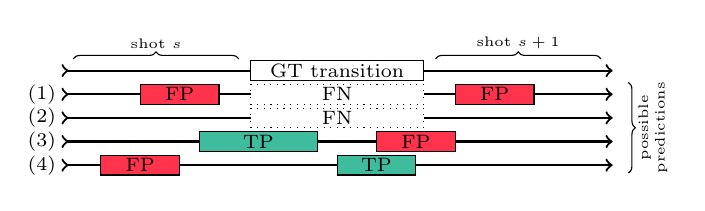
\begin{tikzpicture}
    \definecolor{myred}{RGB}{255,51,76}
    \definecolor{SeaGreen}{RGB}{63,188,157}
    %\definecolor{SeaGreen}{RGB}{208, 240, 192}
    %\definecolor{myred}{RGB}{247, 183, 183}
    
    \draw[decorate,decoration={brace,mirror}] (3.75,.15) -- (1.65,.15) node[midway, anchor=center,sloped, above=0.1, font=\tiny, align=center] {shot $s$};
    \draw[decorate,decoration={brace,mirror}] (8.35,.15) -- (6.25,.15) node[midway, anchor=center,sloped, above=0.1, font=\tiny, align=center] {shot $s+1$};
    
    \draw[>->, thick] (1.5,0) -- (8.5,0);
    \node[draw=black, fill=white, inner sep=0pt, align=center, rectangle,
    minimum width=2.2cm,minimum height=0.25cm, font=\scriptsize] at (5,0) {GT transition};
    
    \node[inner sep=0pt, align=center, font=\scriptsize] at (1.25,-.3) {(1)};
    \draw[>->, thick] (1.5,-.3) -- (8.5,-.3);
    \node[draw=black, fill=myred, inner sep=0pt, align=center, rectangle,
    minimum width=1cm,minimum height=0.25cm, font=\scriptsize] at (3,-.3) {FP};
    \node[draw=black, fill=myred, inner sep=0pt, align=center, rectangle,
    minimum width=1cm,minimum height=0.25cm, font=\scriptsize] at (7,-.3) {FP};
    \node[draw=black, dotted, fill=white, inner sep=0pt, align=center, rectangle,
    minimum width=2.2cm,minimum height=0.25cm, font=\scriptsize] at (5,-.3) {FN};
    
    \node[inner sep=0pt, align=center, font=\scriptsize] at (1.25,-.6) {(2)};
    \draw[>->, thick] (1.5,-.6) -- (8.5,-.6);
    \node[draw=black, dotted, fill=white, inner sep=0pt, align=center, rectangle,
    minimum width=2.2cm,minimum height=0.25cm, font=\scriptsize] at (5,-.6) {FN};
    
    \node[inner sep=0pt, align=center, font=\scriptsize] at (1.25,-.9) {(3)};
    \draw[>->, thick] (1.5,-.9) -- (8.5,-.9);
    \node[draw=black, fill=SeaGreen, inner sep=0pt, align=center, rectangle,
    minimum width=1.5cm,minimum height=0.25cm, font=\scriptsize] at (4,-.9) {TP};
    \node[draw=black, fill=myred, inner sep=0pt, align=center, rectangle,
    minimum width=1cm,minimum height=0.25cm, font=\scriptsize] at (6,-.9) {FP};
    
    \node[inner sep=0pt, align=center, font=\scriptsize] at (1.25,-1.2) {(4)};
    \draw[>->, thick] (1.5,-1.2) -- (8.5,-1.2);
    \node[draw=black, fill=SeaGreen, inner sep=0pt, align=center, rectangle,
    minimum width=1cm,minimum height=0.25cm, font=\scriptsize] at (5.5,-1.2) {TP};
    \node[draw=black, fill=myred, inner sep=0pt, align=center, rectangle,
    minimum width=1cm,minimum height=0.25cm, font=\scriptsize] at (2.5,-1.2) {FP};
    
    
    \draw[decorate,decoration={brace,mirror}] (8.7,-1.3) -- (8.7,-.15) node[midway, anchor=center,sloped, below=0.1, font=\tiny, align=center] {possible\\ predictions};
    
    \end{tikzpicture}

    \caption[Visualization of the evaluation approach]{Visualization of the evaluation approach. Predicted transitions shown with solid and missed with dotted rectangles. Figure taken from \cite{soucek2019transnet}.}
    \label{fig:metricVis}
\end{figure}

\subsection{Training Details}\label{sec:transnetv1TrainDetails}
The training samples are generated on demand by randomly sampling two videos, taking first not yet selected shot from both videos, and joining the shots by a random type of a transition. Only transitions considered for training are hard cuts and dissolves. The position of the transition is generated randomly. For dissolves, also its length is generated randomly from the interval $[5, 30]$.  The length of each training sequence $N$ is selected to be 100 frames. The size of the input frames is set to $48\times 27$ pixels. 

For each frame, the network learns to predict whether there is a transition between the current frame and the next frame. Even in the case of dissolves, when the transition is over multiple frames, the network is trained to predict only the middle frame as a shot boundary. Negative training samples with no transition are not used since the network learns it from the no-transition segments of the input sequence.


The proposed architecture contains the following meta-parameters. We instigate the best meta-parameter setting by a grid search and report the results in Section \ref{sec:transnetV1results}.

\begin{enumerate}
\item $S$ -- the number of DDCNN cells in a SDDCNN block,
\item $L$ -- the number of SDDCNN blocks,
\item $F$ -- the number of filters in the first SDDCNN block (doubled in each following SDDCNN block),
\item $D$ -- the number of neurons in the dense layer.
\end{enumerate}

Prior training, weights are initialized by Glorot initializer \cite{Xavier_Glorot_init}, biases are initialized by zeros. A batch size of 20 was used for all investigated networks. To prevent over-fitting to synthetically generated transitions, the networks are trained only for 30 epochs, each with 300 batches resulting in 180,000 transitions in total. The best model is selected according to its performance on the validation set. We use Adam optimizer \cite{Adam14} with the default learning rate $0.001$ and cross-entropy loss function. Depending on the architecture, the whole training takes approximately two to four hours to complete on a single Tesla V100 GPU.


\subsection{Prediction Details}
The network predicts the likelihood of a transition for all $N=100$ input frames. During validation and testing, only predictions for middle 50 frames are used due to incomplete temporal information for the first/last frames. Therefore, when processing a video, the input window is shifted by 50 frames between individual forward passes through the network. At the start and the end of a video, the first frame and the last frame respectively are duplicated 25 times to pad the video to ensure no unexpected transitions are generated at the video's ends.

For a video, a list of shots is constructed in the following way: A shot starts at the first frame when the predicted likelihood of a transition drops below a threshold $\theta$ and ends at the first frame when the predicted likelihood exceeds~$\theta$. Since the network is trained to predict only one transition frame per any transition, even in case of long dissolves, we lower the acceptance threshold $\theta$ to $0.1$ instead of using the common $0.5$ in all our experiments as it performed reasonably well for most of the models. 


\subsection{Results}\label{sec:transnetV1results}

\begin{table}[b]
	\centering
	\setlength{\tabcolsep}{2.9pt}
	\footnotesize
	\sisetup{detect-weight=true,detect-inline-weight=math}
	\begin{tabular}{l@{\hspace{0.2cm}}S[table-format=2.1]S[table-format=2.1]S[table-format=2.1]S[table-format=2.1]S[table-format=2.1]S[table-format=2.1]S[table-format=2.1]S[table-format=2.1]S[table-format=2.1]S[table-format=2.1]S[table-format=2.1]S[table-format=2.1]S[table-format=2.1]S[table-format=2.1]S[table-format=2.1]}
		\toprule
		\multirow{1}{*}[-1cm]{\textbf{Dataset}} & 
            \multicolumn{1}{c}{\rotatebox[origin=c]{90}{F8 L2 S1 D128}} & 
            \multicolumn{1}{c}{\rotatebox[origin=c]{90}{F8 L2 S2 D128}} & 
            \multicolumn{1}{c}{\rotatebox[origin=c]{90}{F8 L2 S3 D128}} & 
            \multicolumn{1}{c}{\rotatebox[origin=c]{90}{F8 L3 S1 D128}} & 
            \multicolumn{1}{c}{\rotatebox[origin=c]{90}{F8 L3 S2 D128}} & 
            \multicolumn{1}{c}{\rotatebox[origin=c]{90}{F8 L3 S3 D128}} & 
            \multicolumn{1}{c}{\rotatebox[origin=c]{90}{F8 L4 S1 D128}} & 
            \multicolumn{1}{c}{\rotatebox[origin=c]{90}{F8 L4 S2 D128}} & 
            \multicolumn{1}{c}{\rotatebox[origin=c]{90}{F8 L4 S3 D128}} & 
            \multicolumn{1}{c}{\rotatebox[origin=c]{90}{F16 L2 S1 D256}} & 
            \multicolumn{1}{c}{\rotatebox[origin=c]{90}{F16 L2 S2 D256}} & 
            \multicolumn{1}{c}{\rotatebox[origin=c]{90}{F16 L3 S1 D256}} & 
            \multicolumn{1}{c}{\rotatebox[origin=c]{90}{F16 L3 S2 D256}} & 
            \multicolumn{1}{c}{\rotatebox[origin=c]{90}{F16 L4 S1 D256}} & 
            \multicolumn{1}{c}{\rotatebox[origin=c]{90}{F16 L4 S2 D256}} \\
		\midrule
		IACC.3 & 71.0 & 70.9 & 72.0 & 72.0 & 71.7 & 71.6 & 70.4 & 71.4 & 69.5 & \bftabnum 73.4 & 71.6 & \bftabnum 72.7 & \bftabnum 73.1 & 71.6 & 69.9 \\
		RAI    & 92.9 & \bftabnum 94.4 & 93.6 & 93.4 & 93.1 & 93.8 & 93.4 & \bftabnum 94.4 & 91.9 & 92.2 & 93.6 & 91.4 & \bftabnum 94.0 & 91.8 & 92.9 \\
		\bottomrule
	\end{tabular}
	\caption[Meta-parameter grid search results]{Meta-parameter grid search results on validation (IACC.3) and test (RAI) datasets. Reported values are the F1 score in percents with three top-performing models in bold. Data taken from \cite{LokocMM2019}.}
	\label{tb:grid_search_scores}
\end{table}

As already mentioned in Section \ref{sec:transnetv1TrainDetails}, the grid search is performed on four main meta-parameters of the architecture. In Table \ref{tb:grid_search_scores} F1 scores of investigated models are reported for validation (IACC.3) and test (RAI) datasets. Based on the evaluations, the best performing model is considered the one with 16 output filters in every convolution operation in the first SDDCNN block, two DDCNN cells in every one of the three SDDCNN blocks, and with 256 neurons in the dense layer (F=16, L=3 S=2, D=256).

Since the validation dataset contains various sequences of frames where even annotators are not sure whether there is a shot transition, the reported scores for the validation data are lower. Besides, even the top-performing TransNet models face problems with the detection of some transitions, for example, false positives in dynamic shots and false negatives in gradual transitions.
On the validation dataset, the selected model detected 1058 false positives and 679 false negatives with respect to the annotation. This is in contrast to the RAI dataset results reported in Table \ref{tb:resultsRAI}, where the network achieves a lower number of false positives than false negatives. Based on manual inspection of the videos, we conclude that the RAI videos do not contain many highly dynamic shots (i.e. resulting in false positives) compared to the IACC.3 validation set while containing difficult dissolves spanning over dozens of frames (i.e. resulting in false negatives).

The performance comparison of related works is shown in Table \ref{tb:shotDetectors}. The average F1 score $94\%$ of our top-performing model on the RAI dataset is on par with the score reported by Hassanien et al. \cite{Hassanien17}. The overall F1 score even slightly outperforms the work of Hassanien et al., even though they proposed a network with more than 40 times as many parameters trained for a larger set of transition types. Furthermore, our model has the advantage that no additional post-processing is needed.

\begin{figure}
    \centering
    
    \begin{tikzpicture}[/pgfplots/width=\linewidth, /pgfplots/height=\linewidth]
    \begin{axis}[% Axis labels
                 ymin=.8,ymax=1,xmin=0,xmax=1,
    			 % Axis labels
    			 table/col sep=comma,
        		 xlabel={Recall / Threshold},
        		 ylabel={Precision / F1},
         		 xlabel shift={-2pt},
        		 ylabel shift={-3pt},
         		 % General appearance
		         font=\small,
		         axis equal image=true,
		         enlargelimits=false,
		         clip=true,
		         nodes near coords, % Place nodes near each coordinate
		         point meta=explicit symbolic,
		         % Grids 
        	     grid style=dotted, grid=both,
                 major grid style={white!65!black},
        		 minor grid style={white!85!black},
		 		 xtick={0,0.1,...,1.1},
        		 ytick={0,0.1,...,1.1},
         		 minor xtick={0,0.02,...,1},
		         minor ytick={0,0.02,...,1},
        		 % Legend
        		 legend style={at={(0,0)},
                 		       anchor=south west}]
    
    \definecolor{my-red}{RGB}{255,51,76}
    \definecolor{my-blue}{RGB}{25,116,210}

	
	% Human partitions leave-one-out evaluation
    \addplot[my-red,mark size=1.7,thick,mark repeat=10, mark phase=10,mark=*,font=\scriptsize] table[x=Recall,y=Precision, meta index=0] {data/transnetv1-prcurve.txt};
    \addlegendentry{P/R curve}
    \addplot[my-blue,mark size=1.7,thick] table[x=Thr,y=F1] {data/transnetv1-prcurve.txt};
    \addlegendentry{F1/Thr curve}

    \end{axis}
    \end{tikzpicture}
    
    \caption[Performance of the best TransNet model]{Precision/Recall curve for the best performing model with corresponding thresholds $\theta$ next to the points (in red) and F1 score dependency on the threshold (in blue). Measured on the RAI dataset. Figure taken from \cite{soucek2019transnet}.}
    \label{fig:prcurve}
\end{figure}

\begin{table}[b]
    \centering
    \begin{tabular}{|c|c|c|c|c|c|c|c|}
        \hline
        \textbf{Video} & \textbf{\#T}   & \textbf{TP}    & \textbf{FP}    & \textbf{FN}    & \textbf{P}     & \textbf{R}     & \textbf{F1}   \\
        \hline
        V1       &    80 &    57 &     2 &    23 & 96.6 & 71.3 & 82.0\\
        V2       &   146 &   132 &     5 &    14 & 96.4 & 90.4 & 93.3\\
        V3       &   112 &   111 &     4 &     1 & 96.5 & 99.1 & 97.8\\
        V4       &    60 &    59 &     5 &     1 & 92.2 & 98.3 & 95.2\\
        V5       &   104 &   101 &     8 &     3 & 92.7 & 97.1 & 94.8\\
        V6       &    54 &    53 &     3 &     1 & 94.6 & 98.1 & 96.4\\
        V7       &   109 &   103 &     1 &     6 & 99.0 & 94.5 & 96.7\\
        V8       &   196 &   181 &     4 &    15 & 97.8 & 92.3 & 95.0\\
        V9       &    61 &    55 &     2 &     6 & 96.5 & 90.2 & 93.2\\
        V10      &    63 &    57 &     0 &     6 &100.0 & 90.5 & 95.0\\
        \hline
        Overall  &   985 &   909 &    34 &    76 & 96.4 & 92.3 & 94.3\\
        \hline
    \end{tabular}
    
    \caption[Per video results on the RAI dataset]{Per video results on the RAI dataset. For each video, the total number of transitions (\#T), true positives (TP), false positives (FP), false negatives (FN), precision (P), recall (R) and F1 score (F1) are shown. Table taken from \cite{soucek2019transnet}.}
    \label{tb:resultsRAI}
\end{table}


\begin{table}
    \centering
    \begin{tabular}{r|c|c|c|c}
        & Baraldi et al. & Gygli & Hassanien et al. & ours \\
        \hline
        average & 84 \cite{Baraldi15} & 88 \cite{Gygli18} & $\mathbf{94}$ \cite{Hassanien17} & $\mathbf{94}$ \\
        overall & - & - & 93.4 \cite{Hassanien17} & $\mathbf{94.3}$ \\
    \end{tabular}
    
    \caption[Performance comparison of related works on the RAI dataset]{The Average and overall F1 scores for the RAI test dataset of the best architectures. The overall F1 scores are computed by calculating precision and recall over the whole dataset, not just a single video. Table taken from \cite{soucek2019transnet}.}
    \label{tb:shotDetectors}
\end{table}
